\documentclass{article}
\usepackage{a4wide}
\usepackage{xcolor}
\usepackage{tikz}
\usetikzlibrary{scopes}
\usepackage{ifthen}
\usepackage[default]{gfsneohellenic}
\usepackage[LGR,T1]{fontenc}
\usetikzlibrary{shapes}
		
\begin{document}
	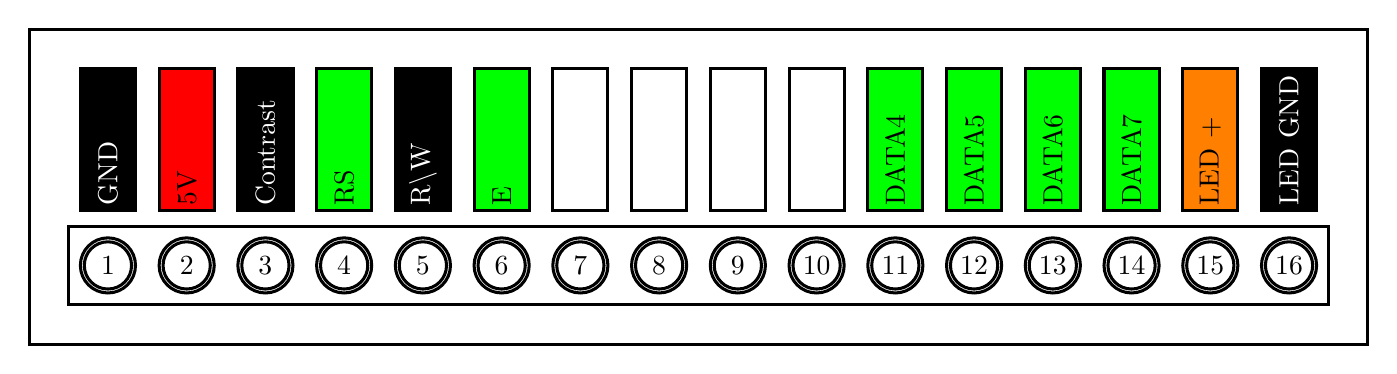
\begin{tikzpicture}[line width=1.1pt]
		\draw(-0.5,-0.5) rectangle (16.5, 3.5);
		\draw(0,0) rectangle (16,1);
		
		\foreach \x in {1,...,16}{
			\draw (\x - 0.5,0.5) node {\x} circle (0.3) circle (0.35);
		}
		
		\draw[fill=black] (0.15,1.2) rectangle (0.85,3);
		\draw[fill=red] (1.15,1.2) rectangle (1.85,3);
		\draw[fill=black] (2.15,1.2) rectangle (2.85,3);
		\draw[fill=green] (3.15,1.2) rectangle (3.85,3);
		\draw[fill=black] (4.15,1.2) rectangle (4.85,3);
		\draw[fill=green] (5.15,1.2) rectangle (5.85,3);
		\draw (6.15,1.2) rectangle (6.85,3);
		\draw (7.15,1.2) rectangle (7.85,3);
		\draw (8.15,1.2) rectangle (8.85,3);
		\draw (9.15,1.2) rectangle (9.85,3);
		\draw[fill=green] (10.15,1.2) rectangle (10.85,3);
		\draw[fill=green] (11.15,1.2) rectangle (11.85,3);
		\draw[fill=green] (12.15,1.2) rectangle (12.85,3);
		\draw[fill=green] (13.15,1.2) rectangle (13.85,3);
		\draw[fill=orange] (14.15,1.2) rectangle (14.85,3);
		\draw[fill=black] (15.15,1.2) rectangle (15.85,3);

		\newcommand{\pinlabel}[2]{%
			\node[anchor=west,rotate=90] at (#1 - 0.5, 1.125) {\ifthenelse{#1 = 1 \OR #1 = 3 \OR #1 = 5 \OR #1 = 16}{\textcolor{white}{#2}}{#2}}
		};
		
		\pinlabel{1}{GND};
		\pinlabel{2}{5V};
		\pinlabel{3}{Contrast};
		\pinlabel{4}{RS};
		\pinlabel{5}{R\textbackslash{}W};
		\pinlabel{6}{E};
		\pinlabel{11}{DATA4};
		\pinlabel{12}{DATA5};
		\pinlabel{13}{DATA6};
		\pinlabel{14}{DATA7};
		\pinlabel{15}{LED +};
		\pinlabel{16}{LED GND};

	\end{tikzpicture}
\end{document}